\chapter{Specifikacija programske potpore}
		
	\section{Funkcionalni zahtjevi}

		\textbf{\textit{dio 1. revizije}}
		
		
		\noindent \textbf{Dionici:}
		
		\begin{packed_enum}
			
			\item Neregistrirani/neprijavljeni korisnik
			\item Spasilac
			\item Doktor(Spasilac)
			\item Vatrogasac(Spasilac)
			\item Policajac(Spasilac)
			\item Voditelj stanice		
			\item Dispečer
			\item Administrator
			\item Razvojni tim
	
			\end{packed_enum}
			
			\noindent \textbf{Akteri i njihovi funkcionalni zahtjevi:}
			
			
			\begin{packed_enum}
				\item \underline{Neregistrirani/neprijavljeni korisnik može:}
				
				\begin{packed_enum}
					
					\item poslati zahtjev za registraciju s željenom ulogom za
					koju se prijavljuje, a potrebni su korisničko ime, fotografija, lozinka, ime, prezime, broj
					mobitela i email adresa\item  \underbar{Akter 1 (inicijator) može:}
					\item prijaviti se za ulogu: 112 dispečer, doktor,
					vatrogasac i policajac
					
				\end{packed_enum}
				
				\item \underline{Spasilac može:}
				
				\begin{packed_enum}
					
					\item osvježiti podatak o dostupnosti za akcije (dostupan i spreman za akciju ili nije)
					\item odazvati se na akciju spašavanja
					
				\end{packed_enum}
				
				\item \underline{Doktor(Spasilac) može:}
				
				\begin{packed_enum}
					
					\item biti osposobljen za vožnju motociklom ili kao putnik u kolima hitne pomoći
					
				\end{packed_enum}
				
				\item \underline{Vatrogasac(Spasilac) može:}
				
				\begin{packed_enum}
					
					\item biti osposobljen za vožnju autocisterni, autoljestvi, zapovjednog vozila i šumskog vozila
					
				\end{packed_enum}
				
				\item \underline{Policajac(Spasilac) može:}
				
				\begin{packed_enum}
					
					\item kretati se kao kontaktni policajac, pomoću motocikla, automobila ili oklopnog vozila
					
				\end{packed_enum}
				
				\item \underline{Voditelj stanice može:}
				
				\begin{packed_enum}
					
					\item definirati koji su spasioci dio njegove stanice
					\item definirati na koji način su spasioci iz njegove stanice osposobljeni voditi spašavanje
					\item odazvati se na akciju spašavanja
					
				\end{packed_enum}
				\item \underline{Dispečer može:}
				
				\begin{packed_enum}
					
					\item na temelju prijave otvarati akcije spašavanja s dostupnim informacijama i fotografijama
					\item vidjeti broj dostupnih spasilaca po stanicama
					\item poslati zahtjev za uključivanjem spasilaca u akciju spašavanja
					\item prilikom slanja zahtjeva definirati na koji način bi spasilac trebao sudjelovati (auto, pješke.. )
					\item definirati razinu hitnosti zahtjeva
					\item ako je potrebno spasioca ukloniti s akcije
					\item ako je akcija spašavanja završila, označiti ju u sustavu kao gotovom
					\item preko karte spasiocima pojedinačno zadati zadatke
					\item pristupiti trenutnim pozicijama svih spasilaca zajedno s prikazom Voronojevog dijagrama
					\item odabrati da se za izradu dijagrama koriste pozicije svih spasioca, ili svih dostupnih neaktivnih spasioca, ili aktivnih spasioca na određenoj akciji
					
				\end{packed_enum}
				\item \underline{Administrator može:}
				
				\begin{packed_enum}
					
					\item vidjeti popis svih registriranih korisnika i njihovih osobnih podataka
					\item potvrditi zahtjeve za registraciju
					\item kreirati stanice
					\item mijenjati dodijeljena prava, osobne podatke i pripadnost stanici
					
				\end{packed_enum}
			\end{packed_enum}
			
			\eject 
			
			
				
			\subsection{Obrasci uporabe}
				
				\textbf{\textit{dio 1. revizije}}
				
				\subsubsection{Opis obrazaca uporabe}
					\textit{Funkcionalne zahtjeve razraditi u obliku obrazaca uporabe. Svaki obrazac je potrebno razraditi prema donjem predlošku. Ukoliko u nekom koraku može doći do odstupanja, potrebno je to odstupanje opisati i po mogućnosti ponuditi rješenje kojim bi se tijek obrasca vratio na osnovni tijek.}\\
					

					\noindent \underbar{\textbf{UC1 -Registracija}}
					\begin{packed_item}
	
						\item \textbf{Glavni sudionik: } Neregistrirani korisnik
						\item  \textbf{Cilj:} Registrirati se
						\item  \textbf{Sudionici:} Baza podataka
						\item  \textbf{Preduvjet:} -
						\item  \textbf{Opis osnovnog tijeka:}
						
						\item[] \begin{packed_enum}
	
							\item Korisnik odabire opciju za se registrirati
							\item Korisnik unosi potrebne podatke
							\item Korisnik dobiva potvrdu da mu je registracija odobrena
						\end{packed_enum}
						
						\item  \textbf{Opis mogućih odstupanja:}
						
						\item[] \begin{packed_item}
	
							\item[2.a] Odabir zauzetog korisničkog imena ili e-mail adrese, unos potrebnih podatak u krivom formatu
							\item[] \begin{packed_enum}
								
								\item Sustav obavještava korisnika o grešci
								\item Korisnik ispravlja podatke ili odustaje od registracije
								
							\end{packed_enum}
							
						\end{packed_item}
					\end{packed_item}
				
					\noindent \underbar{\textbf{UC2 -Prijava}}
					\begin{packed_item}
						
						\item \textbf{Glavni sudionik: } Registrirani korisnik
						\item  \textbf{Cilj:} Dobiti pristup korisničkom sučelju
						\item  \textbf{Sudionici:} Baza podataka
						\item  \textbf{Preduvjet:} Registracija
						\item  \textbf{Opis osnovnog tijeka:}
						
						\item[] \begin{packed_enum}
							
							\item Unos korisničkog imena i lozinke
							\item Pristup korisničkim funkcijama
						\end{packed_enum}
						
						\item  \textbf{Opis mogućih odstupanja:}
						
						\item[] \begin{packed_item}
							
							\item[1.a] Unos krivog korisničkog imena ili lozinke
							\item[] \begin{packed_enum}
								
								\item Sustav obavještava korisnika o grešci
								\item Korisnik ispravlja podatke ili odustaje od registracije
								
							\end{packed_enum}
							
						\end{packed_item}
					\end{packed_item}
			
			
					\noindent \underbar{\textbf{UC3 -Pregled korisnika}}
					\begin{packed_item}
						
						\item \textbf{Glavni sudionik: } Administrator
						\item  \textbf{Cilj:} Vidjeti popis registriranih korisnika i njihove podatke
						\item  \textbf{Sudionici:} Baza podataka
						\item  \textbf{Preduvjet:} Administrator je prijavljen u sustav
						\item  \textbf{Opis osnovnog tijeka:}
						
						\item[] \begin{packed_enum}
							
							\item Administrator odabire opciju pregledavanja korisnika
							\item Prikaže se lista registriranih korisnika s njihovim podacima
						\end{packed_enum}
						
					\end{packed_item}
				
					\noindent \underbar{\textbf{UC4 -Promjena prava i podataka registriranih korisnika}}
					\begin{packed_item}
						
						\item \textbf{Glavni sudionik: } Administrator
						\item  \textbf{Cilj:} Mijenjati prava, podatke i pripadnost stanici registriranih korisnika
						\item  \textbf{Sudionici:} Baza podataka
						\item  \textbf{Preduvjet:} Administrator je prijavljen u sustav
						\item  \textbf{Opis osnovnog tijeka:}
						
						\item[] \begin{packed_enum}
							
							\item Administrator odabire željenog korisnika
							\item Administrator mijenja željene podatke i prava
						\end{packed_enum}
					\end{packed_item}
				
					\noindent \underbar{\textbf{UC5 -Obrada zahtjeva za registraciju}}
					\begin{packed_item}
						
						\item \textbf{Glavni sudionik: } Administrator
						\item  \textbf{Cilj:} Odobriti ili odbiti zahtjev za registraciju
						\item  \textbf{Sudionici:} Baza podataka
						\item  \textbf{Preduvjet:} Administrator je prijavljen u sustav, ima novih zahtjeva za registraciju
						\item  \textbf{Opis osnovnog tijeka:}
						
						\item[] \begin{packed_enum}
							
							\item Administrator odabire opciju pregledavanja zahtjeva za registraciju
							\item Administrator potvrđuje ili odbija registraciju
						\end{packed_enum}
						
					\end{packed_item}
				
					\noindent \underbar{\textbf{UC6 -Kreiranje stanice}}
					\begin{packed_item}
						
						\item \textbf{Glavni sudionik: } Administrator
						\item  \textbf{Cilj:} Napraviti novu stanicu
						\item  \textbf{Sudionici:} Baza podataka
						\item  \textbf{Preduvjet:} Administrator je prijavljen u sustav
						\item  \textbf{Opis osnovnog tijeka:}
						
						\item[] \begin{packed_enum}
							
							\item Administrator odabire opciju stvaranja nove stanice
							\item Administrator unosi potrebne podatke i stvara stanicu
						\end{packed_enum}
						
						
					\end{packed_item}
				
					\noindent \underbar{\textbf{UC7 - \text Osvježavanje dostupnosti}}
					\begin{packed_item}
	
						\item \textbf{Glavni sudionik: }\text Spasilac
						\item  \textbf{Cilj:} \text Ažurirati dostupnost za akciju
						\item  \textbf{Sudionici:} \text Baza podataka
						\item  \textbf{Preduvjet:} \text Spasilac prijavljen
						\item  \textbf{Opis osnovnog tijeka:}
						
						\item[] \begin{packed_enum}
							
							\item \text Spasilac odabire postavke računa
							\item \text Spasilac u svojim postavkama odabire opciju za dostupnost
							\item \text Odabirom jedne od dviju opcija se postavlja dostupnost spasioca
							\item \text Spasilac postaje dostupan ili nedostupan za akciju
						\end{packed_enum}
					\end{packed_item}

					\noindent \underbar{\textbf{UC8 - \text Dodavanje spasilaca }}
					\begin{packed_item}
	
						\item \textbf{Glavni sudionik: }\text Voditelj
						\item  \textbf{Cilj:} \text Dodati spasioca stanici
						\item  \textbf{Sudionici:} \text Baza podataka
						\item  \textbf{Preduvjet:} \text Voditelj prijavljen
						\item  \textbf{Opis osnovnog tijeka:}
						
						\item[] \begin{packed_enum}
	
							\item \text Voditelj odabire opciju pregleda stanice
							\item \text Voditelj dobiva pregled stanice i spasilaca pripadnika stanice
							\item \text Voditelj odabire opciju dodavanja spasilaca
							\item \text Voditelj odabire spasioca iz baze registriranih spasilaca te mu dodjeljuje ulogu
					
						\end{packed_enum}

						\item  \textbf{Opis mogućih odstupanja:}
						
						\item[] \begin{packed_item}
	
							\item[4.a] \text Nema slobodnih spasilaca
							\item[] \begin{packed_item}
								
								\item \text Sustav obavještava voditelja da nema dostupnih spasilaca
								
							\end{packed_item}
							
						\end{packed_item}
						
					\end{packed_item}

					\noindent \underbar{\textbf{UC9 - \text Promjena uloge spasioca }}
					\begin{packed_item}
	
						\item \textbf{Glavni sudionik: }\text Voditelj
						\item  \textbf{Cilj:} \text Promijeniti ulogu spasioca
						\item  \textbf{Sudionici:} \text Baza podataka
						\item  \textbf{Preduvjet:} \text Voditelj prijavljen, spasilac član voditeljeve stanice
						\item  \textbf{Opis osnovnog tijeka:}
						
						\item[] \begin{packed_enum}
	
							\item \text Voditelj odabire opciju pregleda stanice
							\item \text Voditelj dobiva pregled stanice i spasilaca pripadnika stanice
							\item \text Voditelj odabire željenog spasioca
							\item \text Voditelj odabire opciju mijenjanja uloge te ostvaruje tu promjenu
					
						\end{packed_enum}

						\item  \textbf{Opis mogućih odstupanja:}
						
						\item[] \begin{packed_item}
	
							\item[4.a] \text Voditelj nije odabrao niti jednu ulogu
							\item[] \begin{packed_item}
								
								\item \text Sustav obavještava voditelja da nije odabrao ulogu te ga traži da odabere ulogu
								
							\end{packed_item}
							
						\end{packed_item}
						
					\end{packed_item}

					\noindent \underbar{\textbf{UC10 - \text Otvaranje akcije}}
					\begin{packed_item}
	
						\item \textbf{Glavni sudionik: }\text Dispečer
						\item  \textbf{Cilj:} \text Otvoriti akciju i poslati zahtjeve spasiocima
						\item  \textbf{Sudionici:} \text Baza podataka
						\item  \textbf{Preduvjet:} \text Dispečer prijavljen
						\item  \textbf{Opis osnovnog tijeka:}
						
						\item[] \begin{packed_enum}
							
							\item \text Dispečer odabire opciju otvaranja nove akcije
							\item \text Dispečer otvara akciju sa dostupnim informacijama i fotografijama
							\item \text Dispečer dobiva uvid o broju spasilaca po stanicama
							\item \text Dispečer šalje zahtjev pojedinim spasiocima sa definiranim načinom sudjelovanja i hitnosti
						\end{packed_enum}
						
						\item  \textbf{Opis mogućih odstupanja:}
						
						\item[] \begin{packed_item}
	
							\item[2.a] \text Nema dostupnih spasilaca za akciju
							\item[] \begin{packed_item}
								
								\item \text Sustav obavještava dispečera o nedostupnosti spasilaca
								
							\end{packed_item}
							
						\end{packed_item}
					\end{packed_item}

					\noindent \underbar{\textbf{UC11 - \text Završavanje akcije}}
					\begin{packed_item}
	
						\item \textbf{Glavni sudionik: }\text Dispečer
						\item  \textbf{Cilj:}\text Označiti akciju kao završenom
						\item  \textbf{Sudionici:} Baza podataka
						\item  \textbf{Preduvjet:} Akcija završena
						\item  \textbf{Opis osnovnog tijeka:}
						
						\item[] \begin{packed_enum}
	
							\item \text Dispečer odabire završenu akciju
							\item \text Dispečer označava akciju kao završenom
						\end{packed_enum}
						
					\end{packed_item}

					\noindent \underbar{\textbf{UC12 - \text Uklanjanje spasilaca s akcije}}
					\begin{packed_item}
	
						\item \textbf{Glavni sudionik: }\text Dispečer
						\item  \textbf{Cilj:}\text Ukloniti spasioca s akcije
						\item  \textbf{Sudionici:} \text Baza podataka
						\item  \textbf{Preduvjet:} \text Spasilac trenutno na akciji
						\item  \textbf{Opis osnovnog tijeka:}
						
						\item[] \begin{packed_enum}
	
							\item \text Dispečer otvara popis spasilaca na odabranoj akciji
							\item \text Dispečer odabire spasioca te ga miče s akcije
							\item \text Spasilac biva obaviješten o uklanjanju s akcije
						\end{packed_enum}
						
					\end{packed_item}

					\noindent \underbar{\textbf{UC13 - \text Odazivanje na akciju}}
					\begin{packed_item}
	
						\item \textbf{Glavni sudionik: }\text Spasilac
						\item  \textbf{Cilj:} \text Odazivanje na akciju
						\item  \textbf{Sudionici:} \text Baza podataka
						\item  \textbf{Preduvjet:} \text Akcija pokrenuta i dispečer poslao zahtjev spasiocu
						\item  \textbf{Opis osnovnog tijeka:}
						
						\item[] \begin{packed_enum}
	
							\item \text Spasilac dobiva zahtjev od dispečera za uključenje u akciju
							\item \text Spasilac potvrđuje zahtjev ili ga odbija
							\item \text Nakon potvrde vanjski servis izračunava rutu do lokacije
						\end{packed_enum}
						
					\end{packed_item}
				
					\noindent \underbar{\textbf{UC14 - \text Zadavanje pojedinačnih zadataka}}
					\begin{packed_item}
	
						\item \textbf{Glavni sudionik: }\text Dispečer
						\item  \textbf{Cilj:} \text Zadati pojedinačan zadatak spasiocu
						\item  \textbf{Sudionici:} \text Baza podataka, Spasilac
						\item  \textbf{Preduvjet:} \text Spasilac dostupan za akciju
						\item  \textbf{Opis osnovnog tijeka:}
						
						\item[] \begin{packed_enum}
	
							\item \text Dispečer otvara kartu
							\item \text Na karti odabire dostupnog spasioca
							\item \text Dispečer upisuje informacije o zadatku, moguć je zahtjev prolaska određenom rutom do lokacije
							\item \text Dispečer po potrebi dodaje i dodatni komentar
							\item \text Spasilac dobiva informacije o zadatku te izračunatu rutu od strane vanjskog servisa
						\end{packed_enum}
						
						\item  \textbf{Opis mogućih odstupanja:}
						
						\item[] \begin{packed_item}
	
							\item[2.a] \text Nema dostupnih spasilaca za zadatak
							\item[] \begin{packed_item}
								
								\item \text Sustav obavještava dispečera porukom o nedostupnosti spasilaca
								
							\end{packed_item}
							
						\end{packed_item}
					\end{packed_item}		

					\noindent \underbar{\textbf{UC15 - \text Odabir moda izračuna dijagrama}}
					\begin{packed_item}
	
						\item \textbf{Glavni sudionik: }\text Dispečer
						\item  \textbf{Cilj:} \text Odabrati način izračuna Vornojevog dijagrama
						\item  \textbf{Sudionici:} \text Baza podataka, vanjski servis
						\item  \textbf{Preduvjet:} \text Dispečer prijavljen u aplikaciju
						\item  \textbf{Opis osnovnog tijeka:}
						
						\item[] \begin{packed_enum}
							
							\item \text DIspečer odabire opciju pottavki karte
							\item \text Dispečer u postavkama karte odabire opciju "način izračuna"
							\item \text Dispečer odabire jednu od tri opcije:
								\begin{packed_enum}
									\item \text Uključiti sve spasioce
									\item \text Uključiti sve dostupne neaktivne spasioce
									\item \text Uključiti sve spasioce aktivne na određenoj akciji
								\end{packed_enum}
							\item \text Vanjski servis obavlja izračun na temelju odabrane opcije
						\end{packed_enum}
						
					\end{packed_item}	

					\noindent \underbar{\textbf{UC16 - \text Prikaz spasilaca}}
					\begin{packed_item}
	
						\item \textbf{Glavni sudionik: }\text Dispečer
						\item  \textbf{Cilj:} \text Adekvatno prikazati spasioce na karti
						\item  \textbf{Sudionici:} \text Baza podataka
						\item  \textbf{Preduvjet:} \text Dispečer prijavljen u aplikaciju
						\item  \textbf{Opis osnovnog tijeka:}
						
						\item[] \begin{packed_enum}
	
							\item \text Ovisno o ulozi spasioca u akciji, sustav spasioca na karti treba prikazati adekvatnom ikonom
							\item \text Prilikom odabira karte, dispečeru se spasioci koji sudjeluju u akciji prikazuju adekvatnim ikonama
						
						\end{packed_enum}
						
					\end{packed_item}	
				
					\noindent \underbar{\textbf{UC17 -Pregled zadataka}}
					\begin{packed_item}
						
						\item \textbf{Glavni sudionik: } Spasilac
						\item  \textbf{Cilj:} Pregled zadataka koje treba obaviti
						\item  \textbf{Sudionici:} Baza podataka
						\item  \textbf{Preduvjet:} Spasilac je prijavljen u sustav, dispečer je zadao barem jedan zadatak
						\item  \textbf{Opis osnovnog tijeka:}
						
						\item[] \begin{packed_enum}
							
							\item Spasilac pristupa karti na kojoj mu se prikazuju zadaci
							\item moguć je i odabir prikaza popisa svih zadataka
						\end{packed_enum}
						
					\end{packed_item}
					
					\noindent \underbar{\textbf{UC18 -Pregled pozicije ostalih spasilaca}}
					\begin{packed_item}
						
						\item \textbf{Glavni sudionik: } Spasilac
						\item  \textbf{Cilj:} Pregledati trenutnu poziciju ostalih spasilaca aktivnih na istoj akciji
						\item  \textbf{Sudionici:} Baza podataka
						\item  \textbf{Preduvjet:} Spasilac je prijavljen u sustav, ima ostalih spasilaca na istoj akciji
						\item  \textbf{Opis osnovnog tijeka:}
						
						\item[] \begin{packed_enum}
							
							\item Spasilac pristupa karti na kojoj mu se prikazuje lokacija ostalh spasioca
						\end{packed_enum}
						
					\end{packed_item}
					
					\noindent \underbar{\textbf{UC19 -Komentiranje}}
					\begin{packed_item}
						
						\item \textbf{Glavni sudionik: } Spasilac
						\item  \textbf{Cilj:} Ostaviti komentar na karti za ostale sudionike u akciji
						\item  \textbf{Sudionici:} Baza podataka
						\item  \textbf{Preduvjet:} Spasilac je prijavljen u sustav i sudjeluje u akciji
						\item  \textbf{Opis osnovnog tijeka:}
						
						\item[] \begin{packed_enum}
							
							\item  Spasilac pristupa karti te odabire akciju
							\item  Spasilac upisuje svoj komentar o akciji
						\end{packed_enum}
						
					\end{packed_item}
					
					\noindent \underbar{\textbf{UC20 -Pregled komentara}}
					\begin{packed_item}
						
						\item \textbf{Glavni sudionik: } Spasilac
						\item  \textbf{Cilj:} Pregledati komentar ostavljen na karti
						\item  \textbf{Sudionici:} Baza podataka
						\item  \textbf{Preduvjet:} Spasilac je prijavljen u sustav, sudjeluje u akciji i akcija ima ostavljenih komentara
						\item  \textbf{Opis osnovnog tijeka:}
						
						\item[] \begin{packed_enum}
							
							\item  Spasilac pristupa karti te odabire akciju
							\item  Spasilac dobiva uvid u informacije akcije te ostavljene komentare
						\end{packed_enum}
						
					\end{packed_item}	

				\subsubsection{Dijagrami obrazaca uporabe}
					
					\textit{Prikazati odnos aktera i obrazaca uporabe odgovarajućim UML dijagramom. Nije nužno nacrtati sve na jednom dijagramu. Modelirati po razinama apstrakcije i skupovima srodnih funkcionalnosti.}
			
				\begin{figure}[H]
					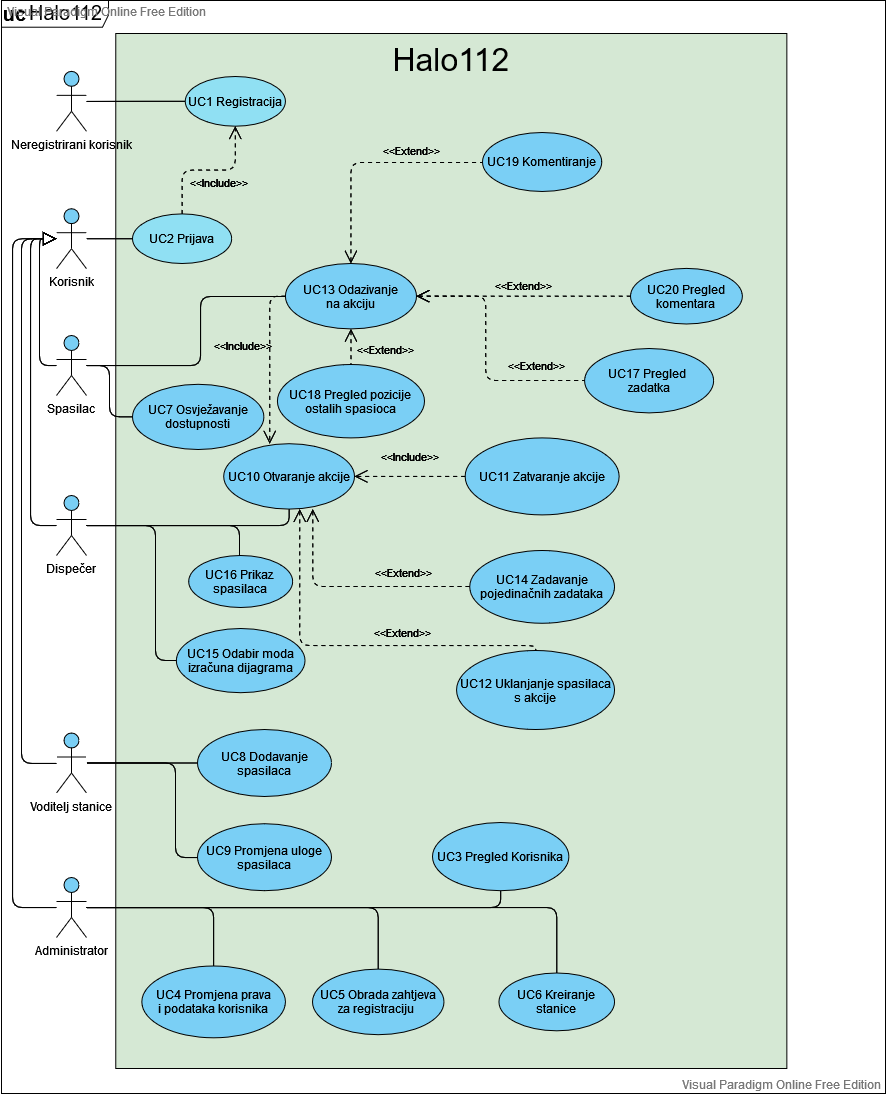
\includegraphics[scale=0.5]{slike/usecase.PNG}
					\centering
					\caption{Dijagram obrazaca uporabe}
					\label{fig:obrasci_uporabe}
				\end{figure}
				\eject		
				
			\subsection{Sekvencijski dijagrami}
				
				\textbf{\textit{dio 1. revizije}}\\
				
				\textit{Nacrtati sekvencijske dijagrame koji modeliraju najvažnije dijelove sustava (max. 4 dijagrama). Ukoliko postoji nedoumica oko odabira, razjasniti s asistentom. Uz svaki dijagram napisati detaljni opis dijagrama.}
				\begin{figure}[H]
					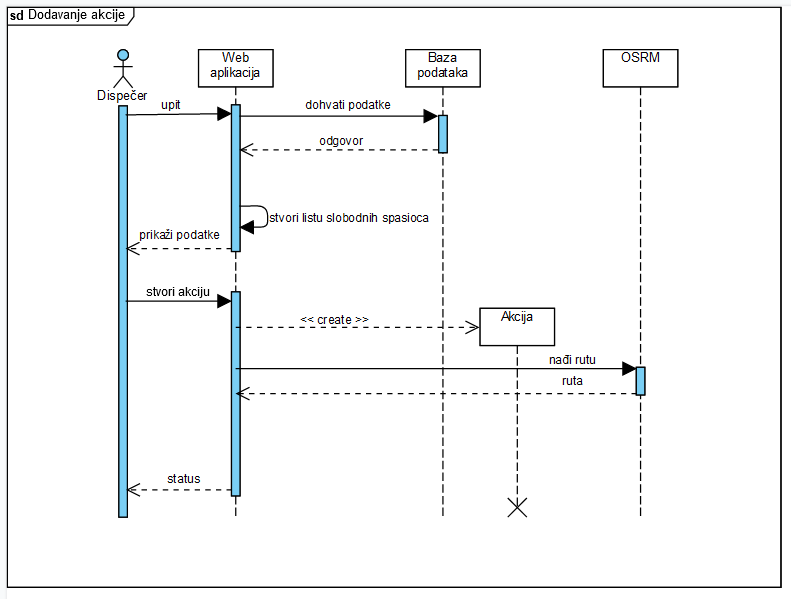
\includegraphics[scale=0.5]{slike/dispatcher_sequence.PNG}
					\centering
					\caption{Sekvencijski dijagram - Otvaranje akcije (UC10)}
					\label{fig:UC10}
				\end{figure}
			
				Prikaz postupka u kojem dispečer stvara akciju i šalje zahtjeve pojedinim spasiocima. Prije stvaranja akcije
				dispečeru se prikazuje popis broja dostupnih spasilaca po stanicama.
			
				\begin{figure}[H]
					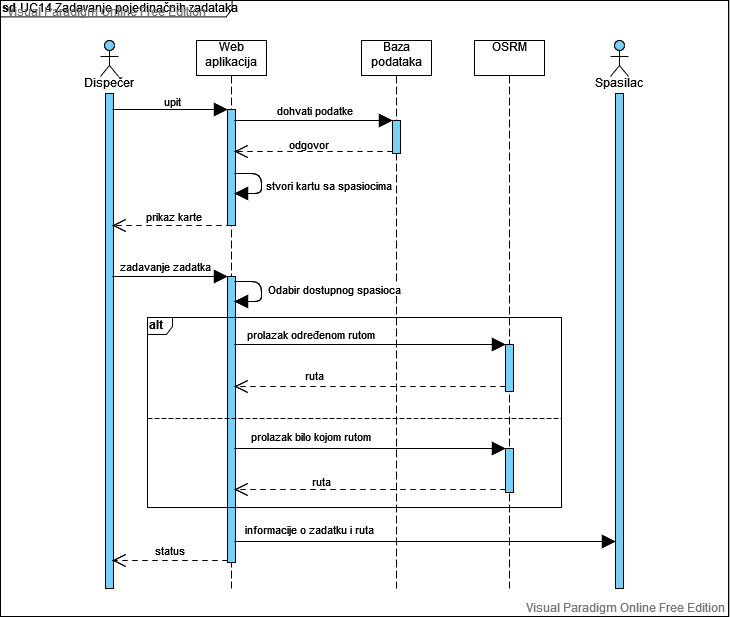
\includegraphics[scale=0.5]{slike/zadavanje_zadataka.png}
					\centering
					\caption{Sekvencijski dijagram - Zadavanje pojedinačnih zadataka (UC14)}
					\label{fig:UC14}
				\end{figure}
				
				Prikaz postupka u kojem dispečer pomoću karte spasilaca zadaje pojedinačni zadatak određenom spasiocu.
				Dispečer može odrediti rutu kojom spasilac prolazi.
				
				\begin{figure}[H]
					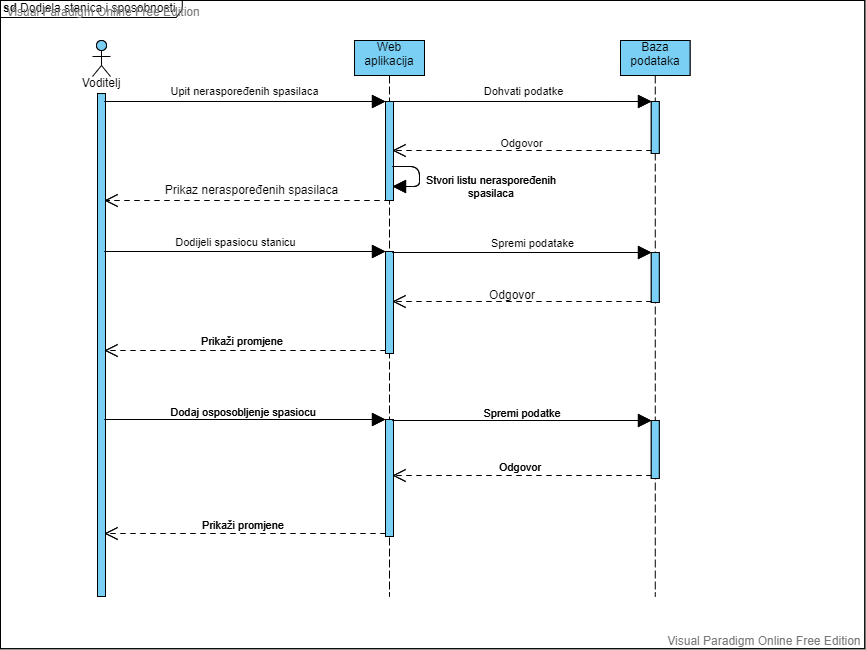
\includegraphics[scale=0.5]{slike/Voditelj.PNG}
					\centering
					\caption{Sekvencijski dijagram - Dodjela stanica i sposobnosti}
					\label{fig:voditelj}
				\end{figure}
			
				Prikaz postupka u kojem voditelj dodaje neraspoređene spasioce u svoju postaju i dodjeljuje im za što su osposobljeni
				
				\begin{figure}[H]
					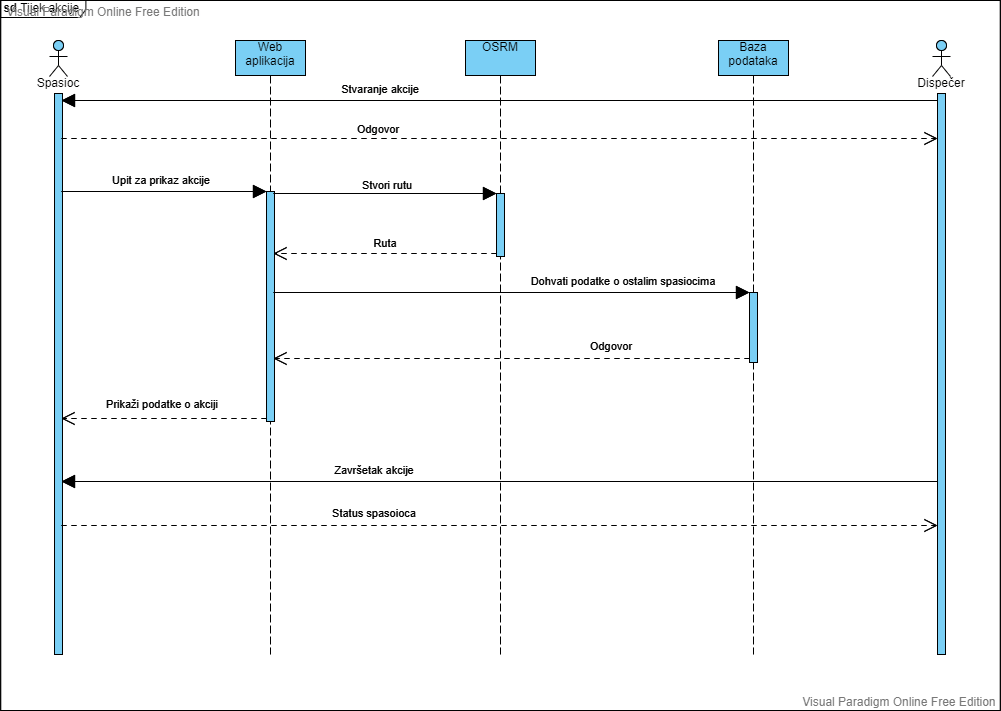
\includegraphics[scale=0.4]{slike/Akcija.PNG}
					\centering
					\caption{Sekvencijski dijagram - Tijek akcije}
					\label{fig:tijekakcije}
				\end{figure}
			
				Prikaz postupka dispečera i spasioca od početka do kraja akcije. Kada je spasiocu dodijeljena akcija, ili on stvara upit za prikaz karte i ostalih sudionika u akciji ili odbija dodijeljenu akciju. kada se spasioc vrati s akcije, dispečer ju zatvara i status spasioca se vraća na dostupan.
				
				\eject
	
		\section{Ostali zahtjevi}
		
			\textbf{\textit{dio 1. revizije}}\\
		 
			 \textit{Nefunkcionalni zahtjevi i zahtjevi domene primjene dopunjuju funkcionalne zahtjeve. Oni opisuju \textbf{kako se sustav treba ponašati} i koja \textbf{ograničenja} treba poštivati (performanse, korisničko iskustvo, pouzdanost, standardi kvalitete, sigurnost...). Primjeri takvih zahtjeva u Vašem projektu mogu biti: podržani jezici korisničkog sučelja, vrijeme odziva, najveći mogući podržani broj korisnika, podržane web/mobilne platforme, razina zaštite (protokoli komunikacije, kriptiranje...)... Svaki takav zahtjev potrebno je navesti u jednoj ili dvije rečenice.}

			
			\begin{packed_item}
			\item  Sustav treba podržavati spajanje više korisnika u vremenu
			\item  Sustav treba biti svima jednostavan za korištenje uz minimalne upute te bez potrebnog korisničkog iskustva
			\item  Korisničko sučelje i sustav moraju podržavati hrvatsku abecedu (dijakritičke znakove) pri unosu i prikazu tekstualnog sadržaja
			\item  Vrijeme odziva treba biti što prije moguće (u nekoliko sekundi)
			\item  Sustav treba biti implementiran kao web aplikacija koristeći objektno-orijentirane jezike
			\item  Neispravno korištenje korisničkog sučelja ne smije narušiti funkcionalnost i rad sustava
			\item  Veza s bazom podataka mora biti kvalitetno zaštićena, brza i otporna na vanjske greške
			\item  Promjene i nadogradnje sustava ne smiju poremetiti rad sustava
			\item  Sustav treba imati ograničen broj spasilaca
			\item  Mjerna jedinica za udaljenost je metar
			 \end{packed_item}
			 
			 
	